\documentclass[a4paper]{article}

\usepackage[utf8]{inputenc}
\usepackage[T1]{fontenc}
\usepackage[polish, english]{babel}
\usepackage{lmodern}
\usepackage{csquotes}

\usepackage[a4paper,top=2cm,bottom=2cm,left=1.5cm,right=1.5cm,marginparwidth=1.75cm]{geometry}
\usepackage{parskip}

\usepackage{microtype}
\usepackage{xcolor}

\usepackage{caption}
\captionsetup{font=small, labelfont=bf, skip=5pt}
\usepackage{subcaption}

\usepackage{amsmath, amssymb, wasysym}
\usepackage{pgfplots}
\pgfplotsset{compat=1.18}
\usepackage{graphicx}
\usepackage{tikz}
\usepackage{tikz-3dplot}
\usepackage{float}
\usepgfplotslibrary{fillbetween}
\usetikzlibrary{intersections}

\usepackage{tcolorbox}
\tcbset{
    colframe=blue!70,
    colback=blue!10,
    arc=5mm,
    boxrule=1pt,
    width=\textwidth,
    sharp corners=downhill,
    fonttitle=\bfseries
}
\newtcolorbox{usefulfactbox}[1][]{title=Przydatny fakt,#1}
\newtcolorbox{solutionbox}{
    colframe=black,
    colback=gray!10,
    arc=10pt,
    boxrule=1pt,
    width=\textwidth,
    top=5pt, bottom=5pt,
    left=5pt, right=5pt,
}

\usepackage{listings}
\usepackage{courier}
\lstdefinelanguage{SAS}{
    morekeywords={data, set, proc, run, if, then, else, do, end, output, input, put, format, informat, length, where, merge, by, retain, drop, keep, label, title, footnote},
    sensitive=false,
    morecomment=[l]{*},
    morecomment=[n]{/*}{*/},
    morestring=[b]",
    morestring=[b]'
}
\lstset{
    language=SAS,
    basicstyle=\footnotesize\ttfamily,
    keywordstyle=\color{blue}\bfseries,
    commentstyle=\color{gray}\itshape,
    stringstyle=\color{red},
    breaklines=true,
    showstringspaces=false,
    frame=single,
    rulecolor=\color{black},
    backgroundcolor=\color{white},
    tabsize=4,
    captionpos=b
}

\usepackage{fancyhdr}
\usepackage[colorlinks=true, linkcolor=blue, pdftitle={Tęczówka oka}, pdfauthor={Michał Matuszyk, Paweł Pozorski}]{hyperref}
\pagestyle{fancy}
\fancyhf{}
\fancyfoot[C]{\thepage}
\renewcommand{\headrulewidth}{0pt}

\usepackage{cleveref}

\title{\textbf{Tęczówka oka}\\[0.5em]}
\author{Michał Matuszyk, Paweł Pozorski}
\date{Kwiecień 2025}

\begin{document}

\maketitle

\begin{abstract}
W niniejszym projekcie zrealizowano pełną ścieżkę przetwarzania obrazu tęczówki oka w celu wygenerowania charakterystycznego „kodu tęczówki” zgodnie z podejściem zaproponowanym przez Johna Daugmana. Przeprowadzone testy wstępne potwierdziły poprawność działania algorytmu oraz wykazały obiecujące rezultaty w kontekście zastosowań biometrycznych.
\end{abstract}

\newpage

\tableofcontents
\newpage

\section{Wprowadzenie}

\subsection*{Demonstracja całego procesu}

Najciekawsze etapy procesu są zilustrowane na \Cref{fig:skrot-procesu}.

Pierwszym etapem jest \textbf{dokładna segmentacja tęczówki}.  
Proces ten musi być odporny na odbicia światła, zmienny kąt rejestracji czy różnorodne rozmiary źrenicy, dlatego wymaga starannego doboru filtrów i progów.

Po wyznaczeniu brzegów tęczówki obraz zostaje \textbf{przetransformowany ze współrzędnych biegunowych do kartezjańskich}.  
Rozwinięty pierścień dzieli się na \textbf{osiem poziomych pasów}, z których każdy podlega selektywnemu przycięciu, tak aby usunąć fragmenty zniekształcone lub pozbawione informacji.

Następnie pasy są \textbf{skomprymowane} do rozmiaru \(1 \times 128\;\text{px}\) (szerokość × wysokość), co stabilizuje rozdzielczość wejściową i upraszcza dalsze obliczenia.

Na tak przygotowanych danych uruchamiany jest \textbf{algorytm Daugmana}, który przy użyciu filtrów Gabora generuje binarny \emph{kod tęczówki} – końcowy, zwarty i porównywalny pomiędzy osobami.

\begin{figure}[H]
    \centering
    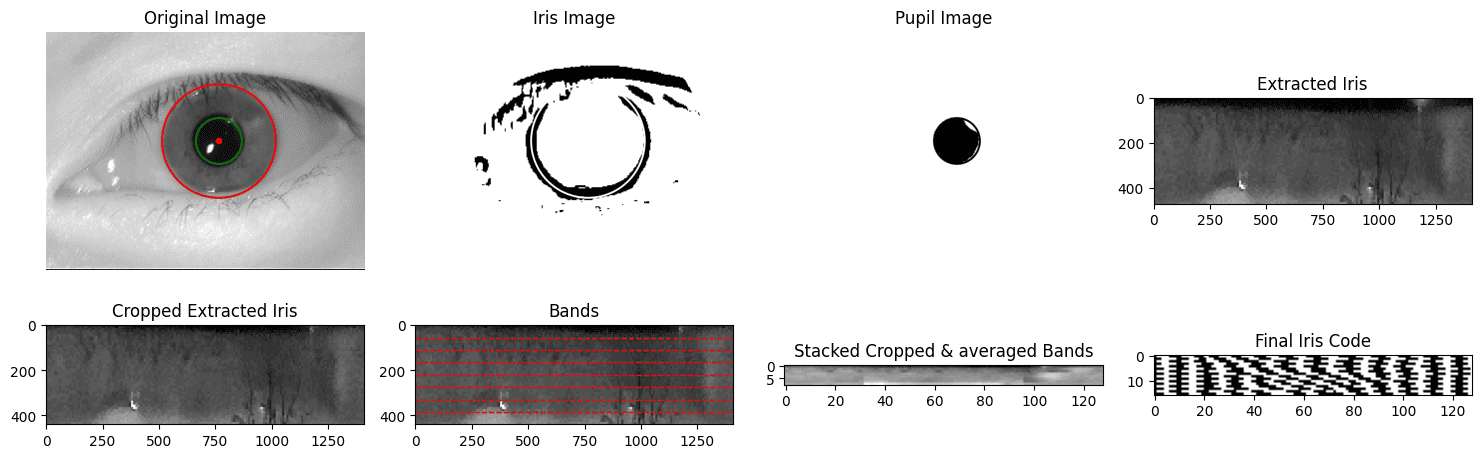
\includegraphics[width=0.75\linewidth]{figures/entire_process.png}
    \caption{Skrótowy pokaz całego procesu}
    \label{fig:skrot-procesu}
\end{figure}

\clearpage

\section{Przygotowanie obrazu tęczówki}

\subsection{Zbiór danych}
Zbiór danych tęczówek wykorzystany w analizie pochodzi z platformy Kaggle i nosi nazwę \emph{naureenmohammad/mmu-iris-dataset}. Zawiera on zdjęcia oczu (prawego i lewego) pochodzące od 45 osób, z których każde oko zostało sfotografowane pięciokrotnie. Niestety, zdjęcia cechują się jedynie przeciętną jakością – w wielu przypadkach znaczna część tęczówki jest przesłonięta przez powiekę. Przykład takiej sytuacji przedstawiono na \Cref{fig:powieka_zakrywa_teczowke}, gdzie fragment tęczówki jest zakryty zarówno od góry, jak i od dołu. Przykład 10 zdjęć pochodzących od jednej osoby jest widoczny na \Cref{fig:przyklady-teczowek}. Jak widać, zdjęcia różnią się między sobą i rzadko źrenica jest na środku.

\begin{figure}[H]
    \centering
    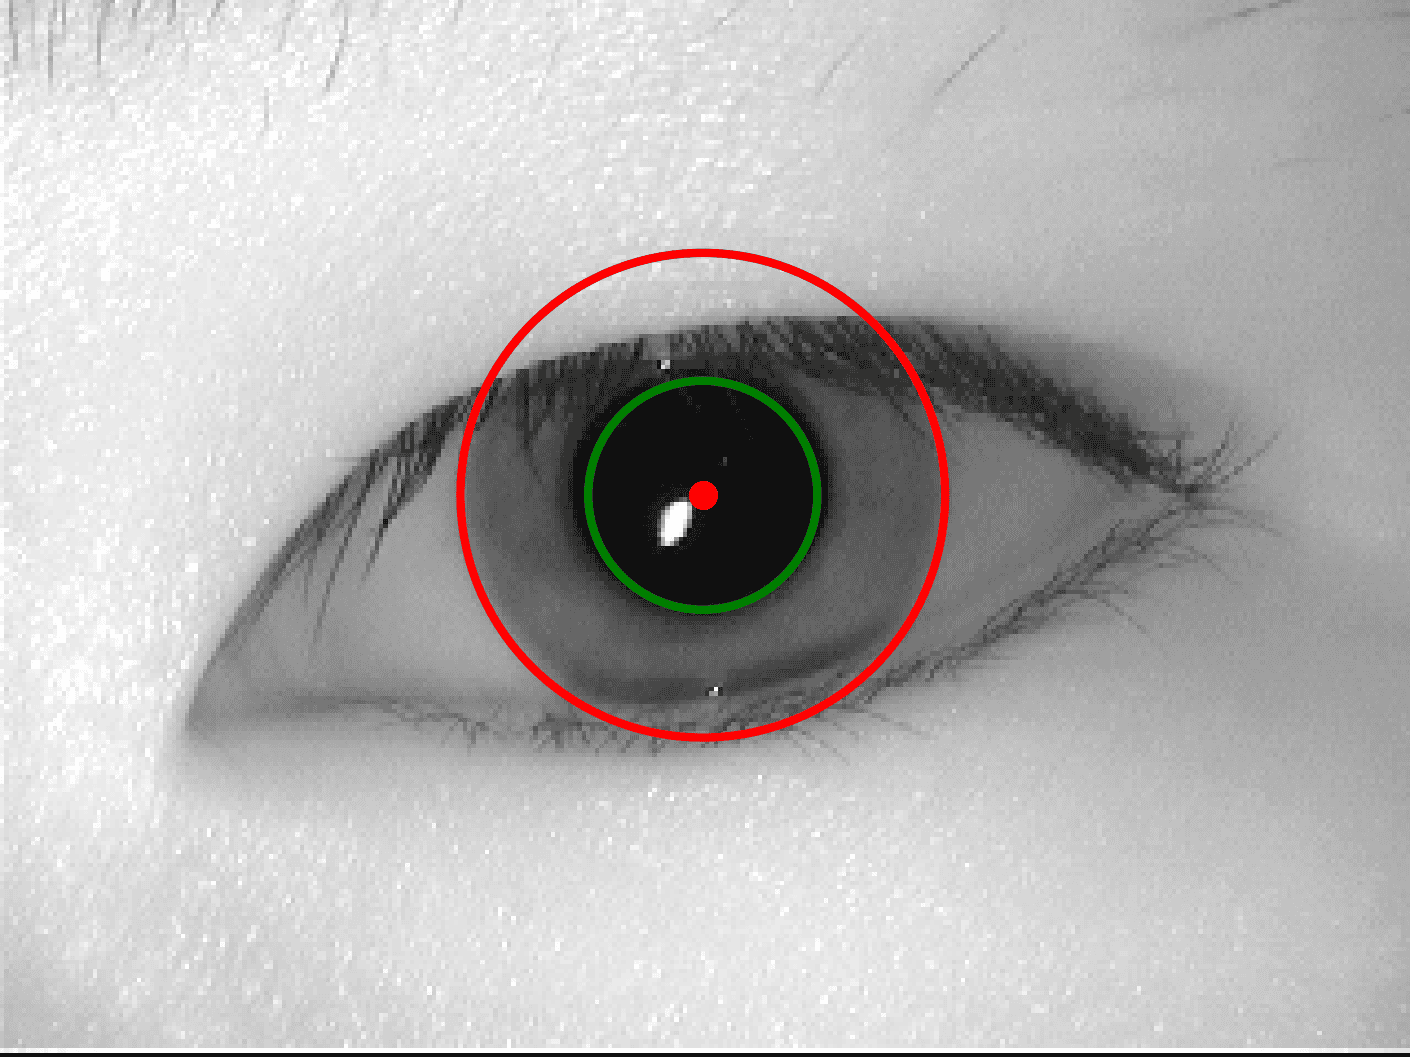
\includegraphics[width=0.3\linewidth]{figures/zdj_zakryte_powieka.png}
    \caption{Znaczna część tęczówki jest zakryta przez powiekę zarówno górną jak i dolną.}
    \label{fig:powieka_zakrywa_teczowke}
\end{figure}

\begin{figure}[H]
    \centering
    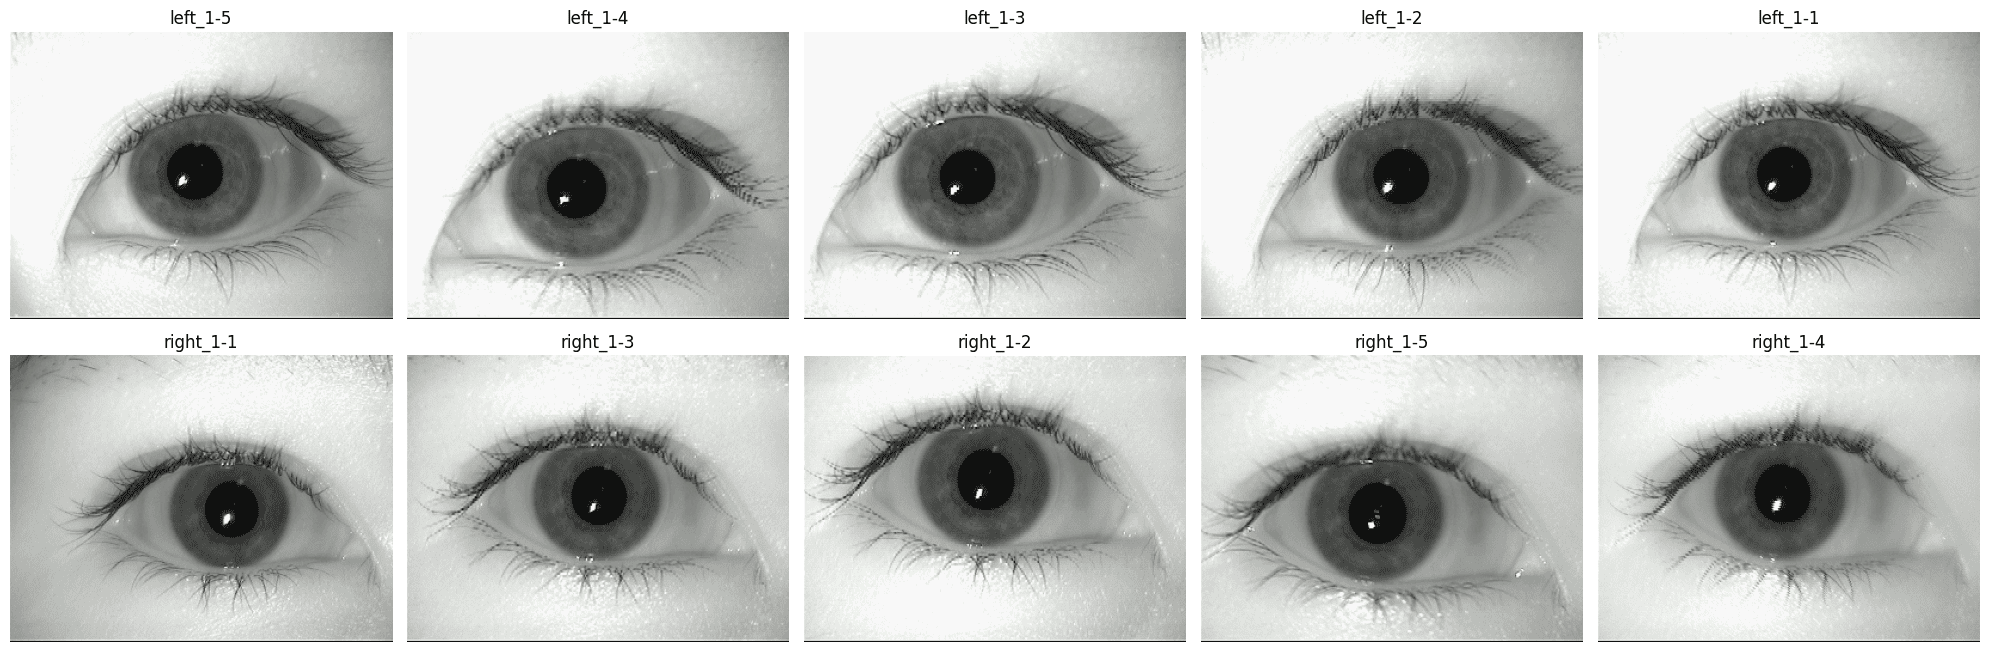
\includegraphics[width=0.75\linewidth]{figures/przyklady teczowek.png}
    \caption{Przykłady tęczówek}
    \label{fig:przyklady-teczowek}
\end{figure}

\subsection{Detekcja granic źrenicy}
Detekcja granic źrenicy stanowi kluczowy etap wstępnego przetwarzania obrazu tęczówki. W badaniu zastosowano proste podejście progowe, oparte na średniej jasności obrazu. Dla każdego obrazu obliczana jest średnia wartość piksela, a następnie stosowane są różne wartości progowe będące jej ułamkami, co umożliwia segmentację potencjalnego obszaru źrenicy. Przykład działania tej metody przedstawiono na \Cref{fig:pupil_thresholds}, gdzie widoczne są wyniki progowania obrazu dla różnych wartości progowych.

\begin{figure}[H]
    \centering
    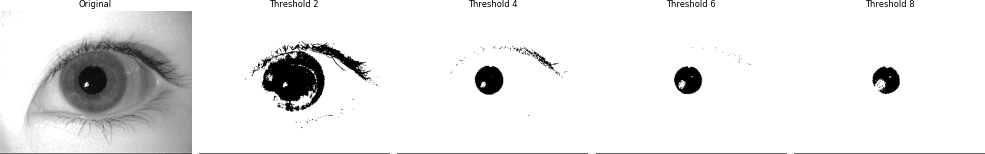
\includegraphics[width=0.9\linewidth]{figures/pupil_thresholds.png}
    \caption{Przykład progowania obrazu w celu detekcji źrenicy dla różnych wartości progów.}
    \label{fig:pupil_thresholds}
\end{figure}

Dla lepszego zobrazowania działania algorytmu, na ilustracji \Cref{fig:pupil_thresholds_many} przedstawiono efekty progowania dla losowo wybranych obrazów. Widać, że skuteczność detekcji zależy od jakości obrazu oraz parametrów progowania.

\begin{figure}[H]
    \centering
    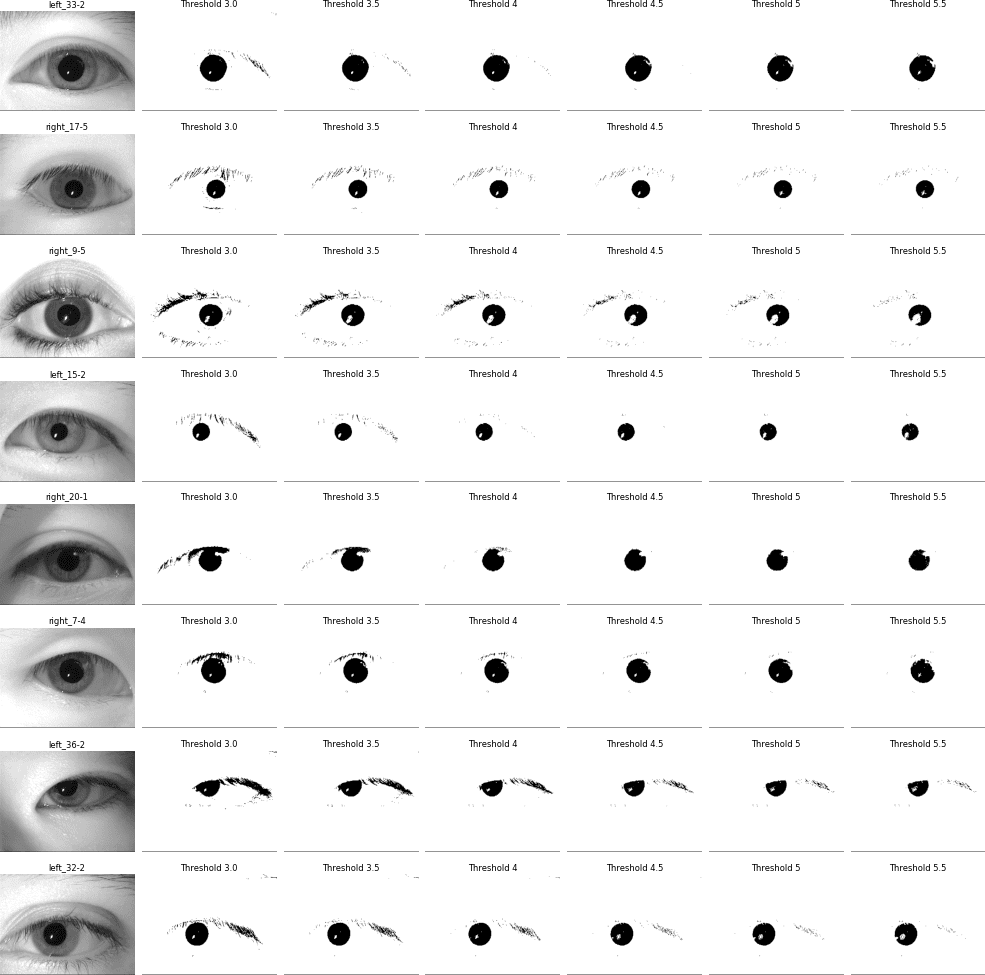
\includegraphics[width=0.9\linewidth]{figures/pupil_thresholds_many.png}
    \caption{Progowanie źrenicy dla różnych zdjęć i progów.}
    \label{fig:pupil_thresholds_many}
\end{figure}

W celu poprawy jakości detekcji źrenicy, zastosowano filtr wyostrzający w połączeniu z regulacją kontrastu. Wyniki tej operacji pokazano na \Cref{fig:eye_filters_many}. Zmodyfikowane obrazy wykazują większy kontrast w obszarze źrenicy, co umożliwia dokładniejsze wyznaczenie jej granic.

\begin{figure}[H]
    \centering
    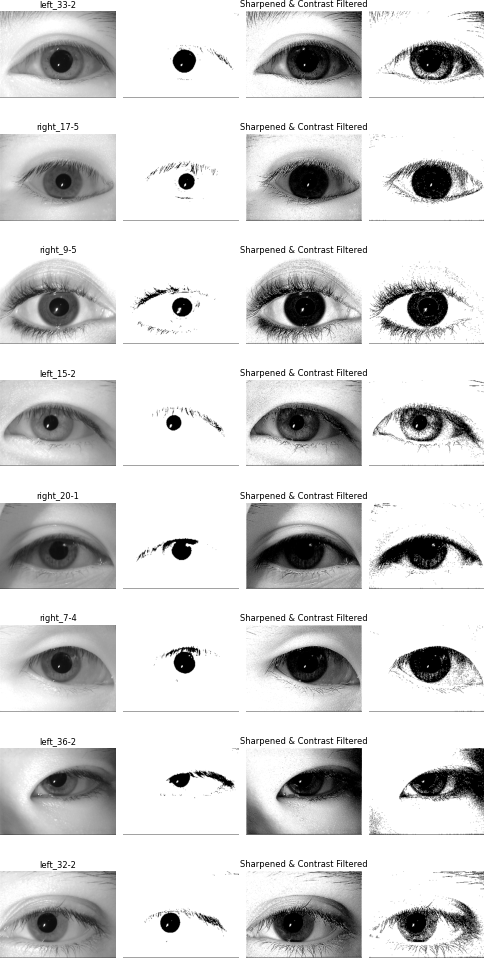
\includegraphics[width=0.7\linewidth]{figures/eye_filters_many.png}
    \caption{Zastosowanie filtrów poprawiających kontrast oraz wyostrzenie obrazu dla lepszej segmentacji źrenicy.}
    \label{fig:eye_filters_many}
\end{figure}

Następnie, dla zsegmentowanych binarnych obrazów źrenicy, wykonano projekcje pionowe i poziome, co pozwala na wyznaczenie środka źrenicy oraz jej przybliżonego promienia. Na ilustracji \Cref{fig:pupils_projections_many} przedstawiono wyniki projekcji wraz z oznaczeniem centrum oraz obszaru źrenicy.

\begin{figure}[H]
    \centering
    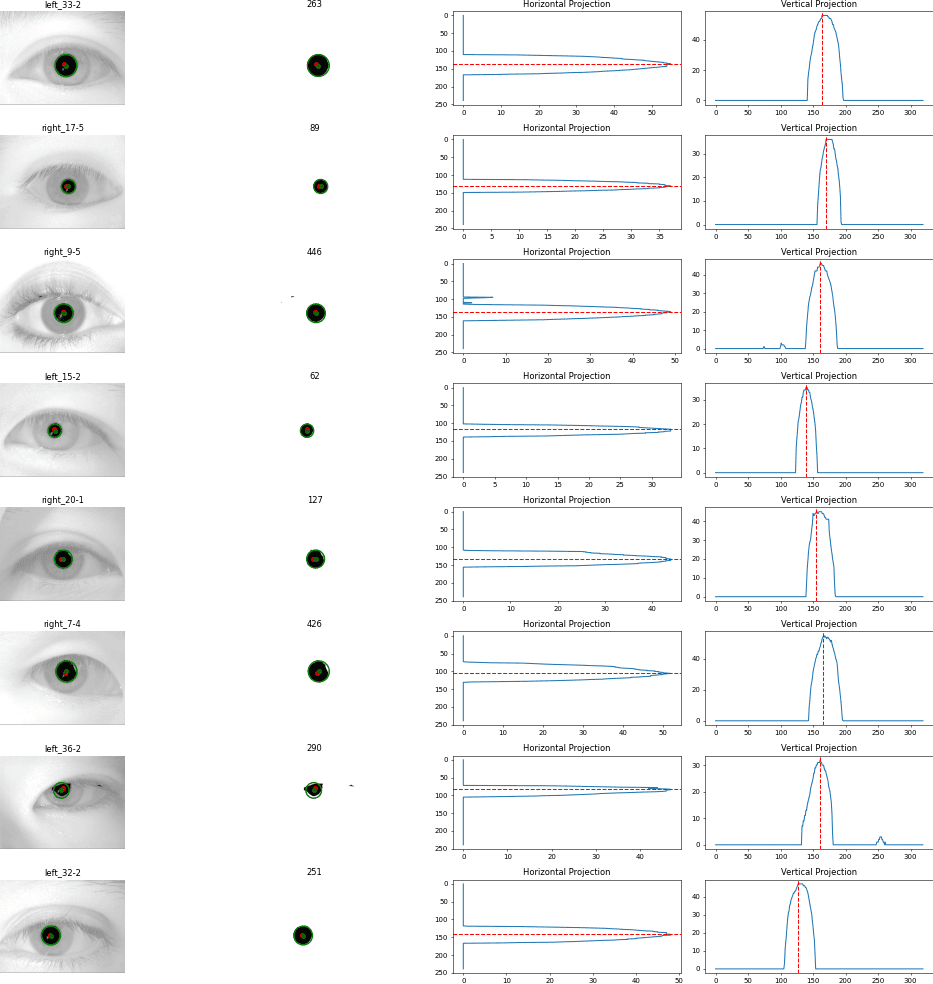
\includegraphics[width=0.9\linewidth]{figures/pupils_projections_many.png}
    \caption{Wizualizacja projekcji poziomych i pionowych dla określenia środka i promienia źrenicy.}
    \label{fig:pupils_projections_many}
\end{figure}

Ostateczny rezultat detekcji źrenicy, wraz z naniesionym środkiem i promieniem, zaprezentowano na ilustracji \Cref{fig:pupils_detected_many}. Rysowane okręgi reprezentują wykrytą granicę źrenicy dla różnych obrazów w zbiorze danych. W niektórych przypadkach granice źrenic mogą wydawać się trochę mniejsze od rzeczywistych granic, co wynika z zastosowania operacji morfologicznych. Eksperymenty niezawarte w tym sprawozdaniu wykazały jednak wyżość takiego rozwiązania nad rozwiązaniami dokładnie wyznaczającymi granicę dla zbioru danych "MMU Iris Dataset", ponieważ zdjęcia w nim zawarte mają w wielu przypadkach wyraźne refleksy świetlne zaburzające powodującą błędy w dokładnej detekcji.

\begin{figure}[H]
    \centering
    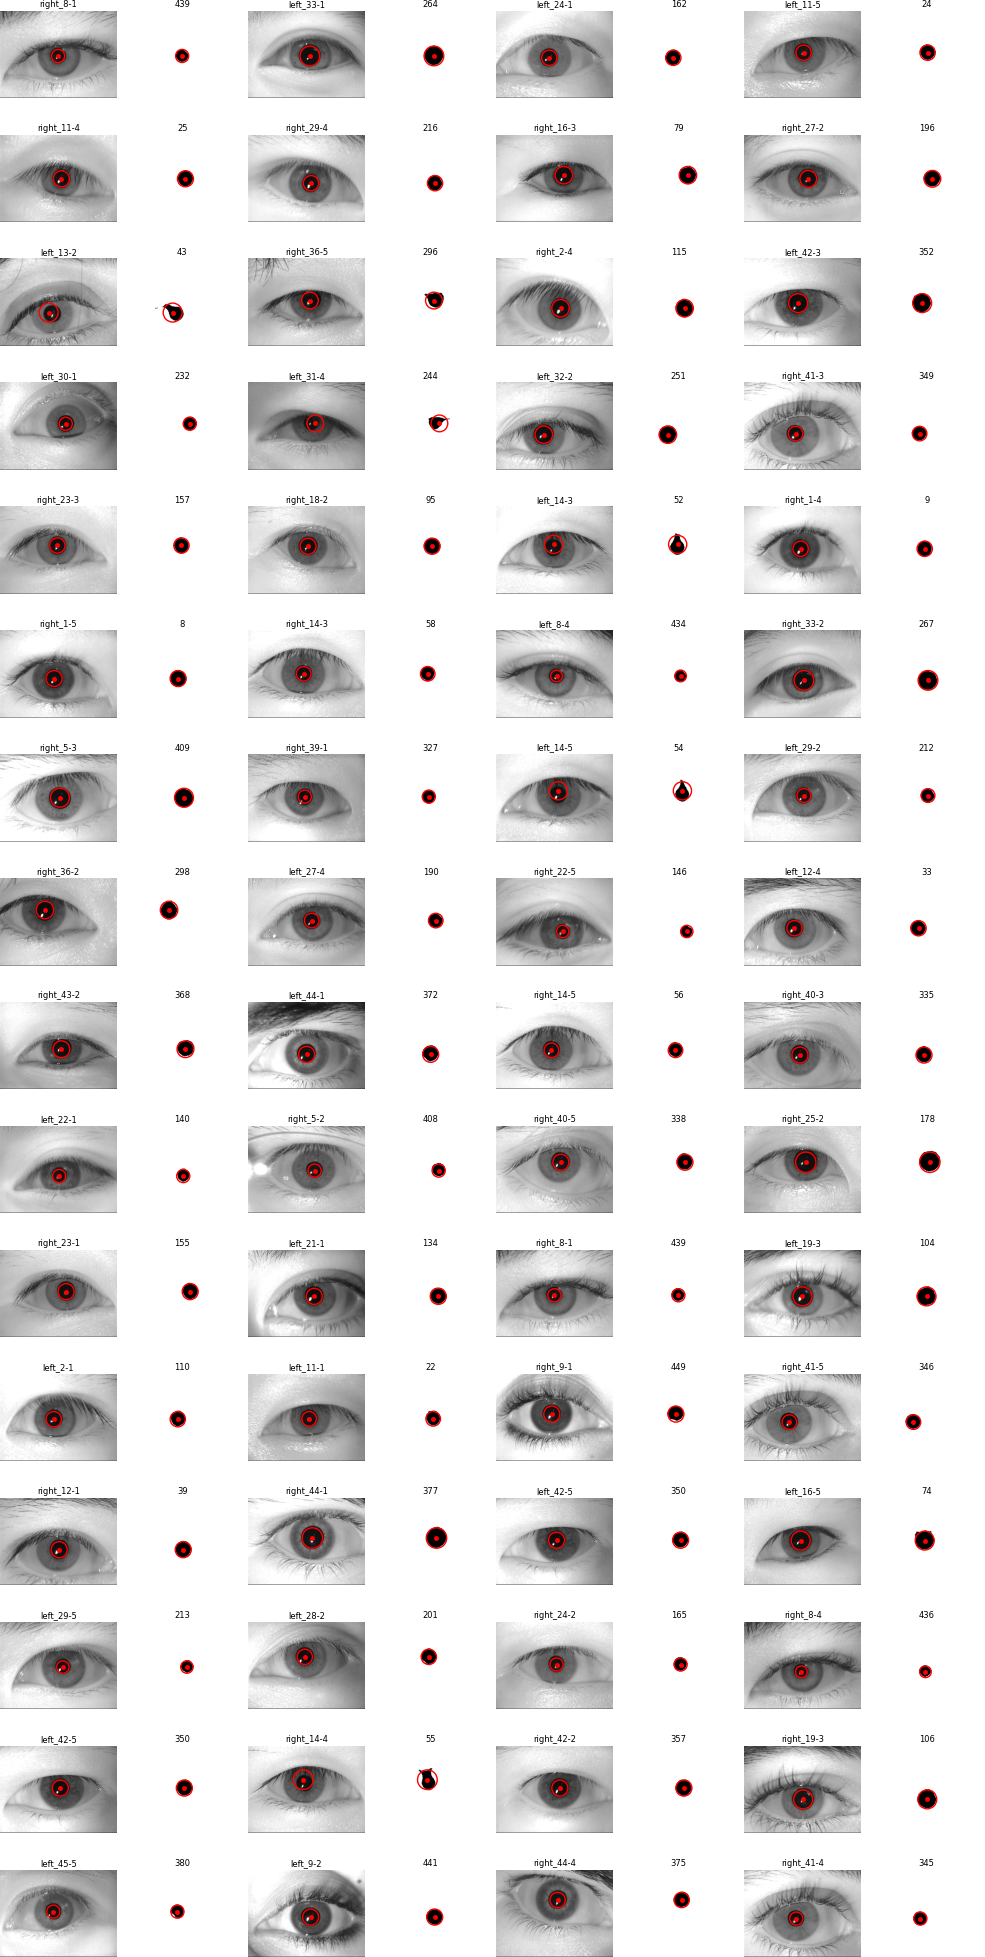
\includegraphics[width=0.9\linewidth]{figures/pupils_detected_many.png}
    \caption{Wykrycie źrenicy – środek oraz promień zaznaczone na obrazach źrenicy.}
    \label{fig:pupils_detected_many}
\end{figure}

\subsection{Detekcja granic tęczówki}
Po wyznaczeniu granic źrenicy kolejnym etapem jest detekcja granic tęczówki. W tym celu wykorzystano kombinację filtrów: wygładzającego (średniego), kontrastowego oraz filtru Sobela, który umożliwia uwidocznienie krawędzi na obrazie. Przykładowe przekształcenia oraz wyniki binarnej segmentacji obrazu po filtracji przedstawiono na ilustracji \Cref{fig:irises_detection_many}.

\begin{figure}[H]
    \centering
    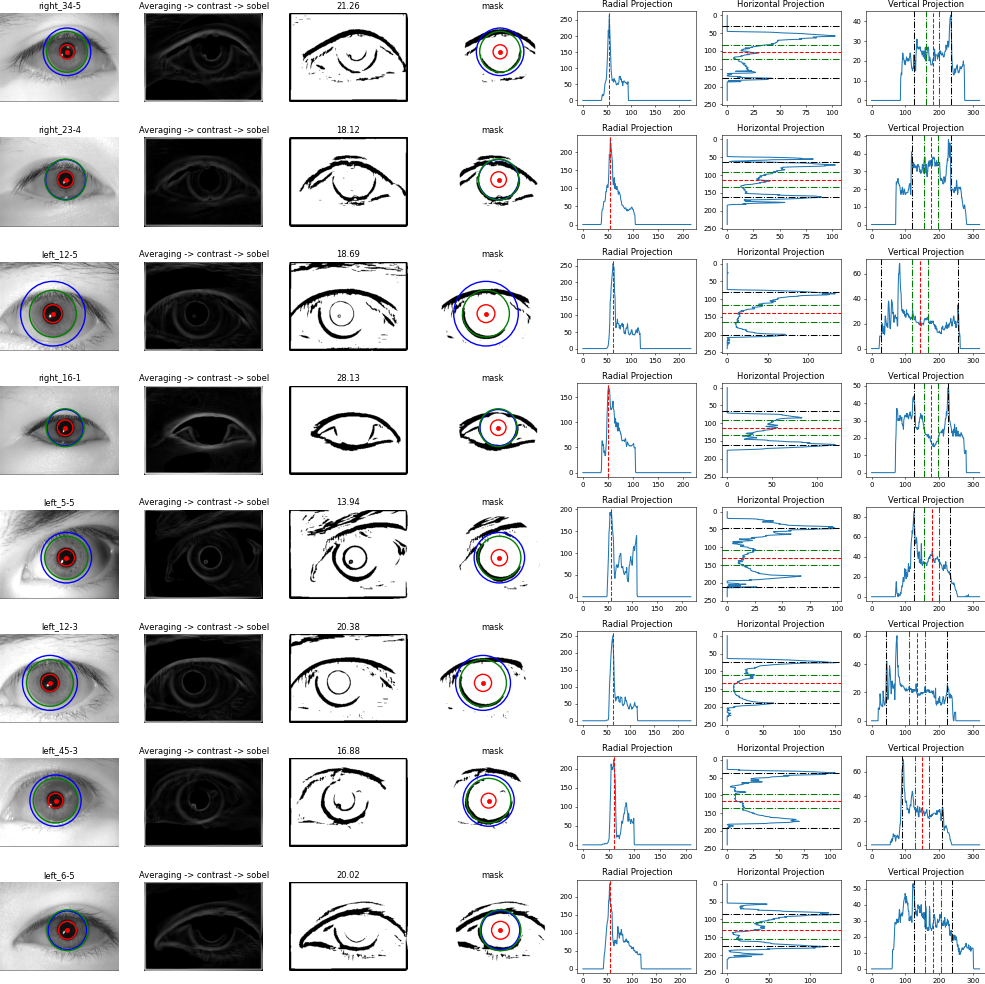
\includegraphics[width=0.95\linewidth]{figures/irises_detection_many.png}
    \caption{Etapy detekcji tęczówki: przekształcenie obrazu, segmentacja, maskowanie oraz wyznaczenie promienia tęczówki na podstawie trzech projekcji.}
    \label{fig:irises_detection_many}
\end{figure}

Po przetworzeniu obrazu zastosowano binarny próg względem średniej wartości pikseli, a następnie maskowanie zbędnych obszarów: przy brzegach kadru oraz wokół źrenicy. Dzięki temu możliwe było ograniczenie wpływu tła oraz refleksów świetlnych.

Kolejnym krokiem była analiza trzech typów projekcji: poziomej, pionowej oraz radialnej. Projekcja radialna obliczana względem środka źrenicy pozwoliła oszacować promień tęczówki w najbardziej bezpośredni sposób. Jednocześnie promienie wyznaczane z projekcji poziomej i pionowej pozwalały na korektę i uśrednienie wartości. Końcowy promień tęczówki określono jako średnią z promieni uzyskanych metodą projekcyjną (pionową i poziomą).

Na rysunkach zaznaczono granice zarówno źrenicy (kolor czerwony), jak i tęczówki – promień obliczony z projekcji radialnej (zielony) oraz średni promień z analiz poziomej i pionowej (niebieski).

Dla wizualizacji końcowego efektu detekcji, przygotowano ilustrację \Cref{fig:irises_detected_many}, gdzie widoczne są zarówno oryginalne obrazy tęczówek, jak i ich binarne odpowiedniki z zaznaczonymi granicami.

\begin{figure}[H]
    \centering
    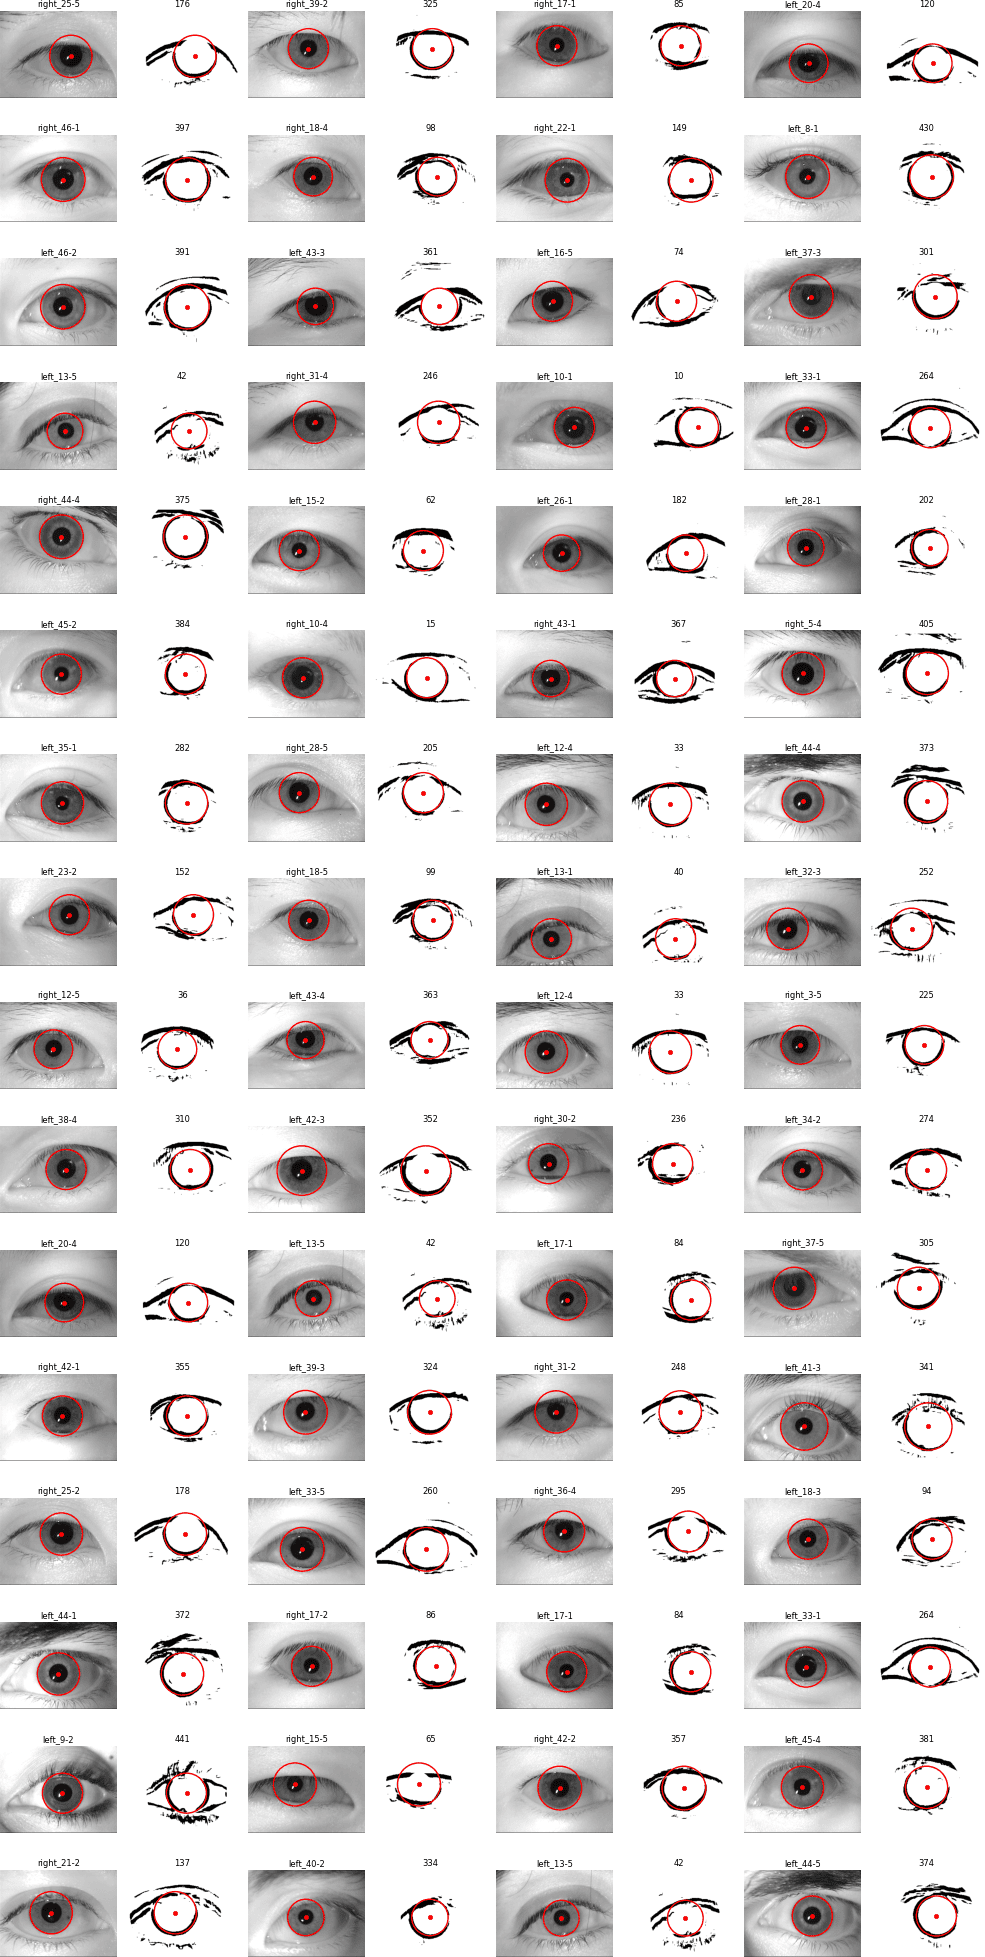
\includegraphics[width=0.7\linewidth]{figures/irises_detected_many.png}
    \caption{Ostateczne wykrycie granic tęczówek w zestawie danych. Pokazano oryginalne obrazy oraz odpowiadające im segmentacje z zaznaczoną granicą tęczówki.}
    \label{fig:irises_detected_many}
\end{figure}

\subsection{Ekstrakcja tęczówki}
Po detekcji granic źrenicy i tęczówki kolejnym krokiem jest wyizolowanie samego obszaru tęczówki w celu dalszej analizy. Proces ten polega na wycięciu pierścienia znajdującego się pomiędzy granicami źrenicy i tęczówki. Przykładowy przebieg tej operacji przedstawiono na ilustracji \Cref{fig:final_comparison}.

Na każdej z wizualizacji zaprezentowano:
\begin{itemize}
    \item oryginalny obraz oka wraz z zaznaczonymi granicami źrenicy (kolor zielony) i tęczówki (kolor czerwony),
    \item obraz binarny z obszarem tęczówki,
    \item obraz binarny z obszarem źrenicy,
    \item oraz wyodrębniony pierścień tęczówki przekształcony do formy prostokątnej (\textit{unwrapped annular segment}).
\end{itemize}

Przekształcenie polega na rozprostowaniu pierścienia tęczówki na obraz prostokątny – proces ten ułatwia późniejsze etapy analizy i porównywania struktur tęczówek.

\begin{figure}[H]
    \centering
    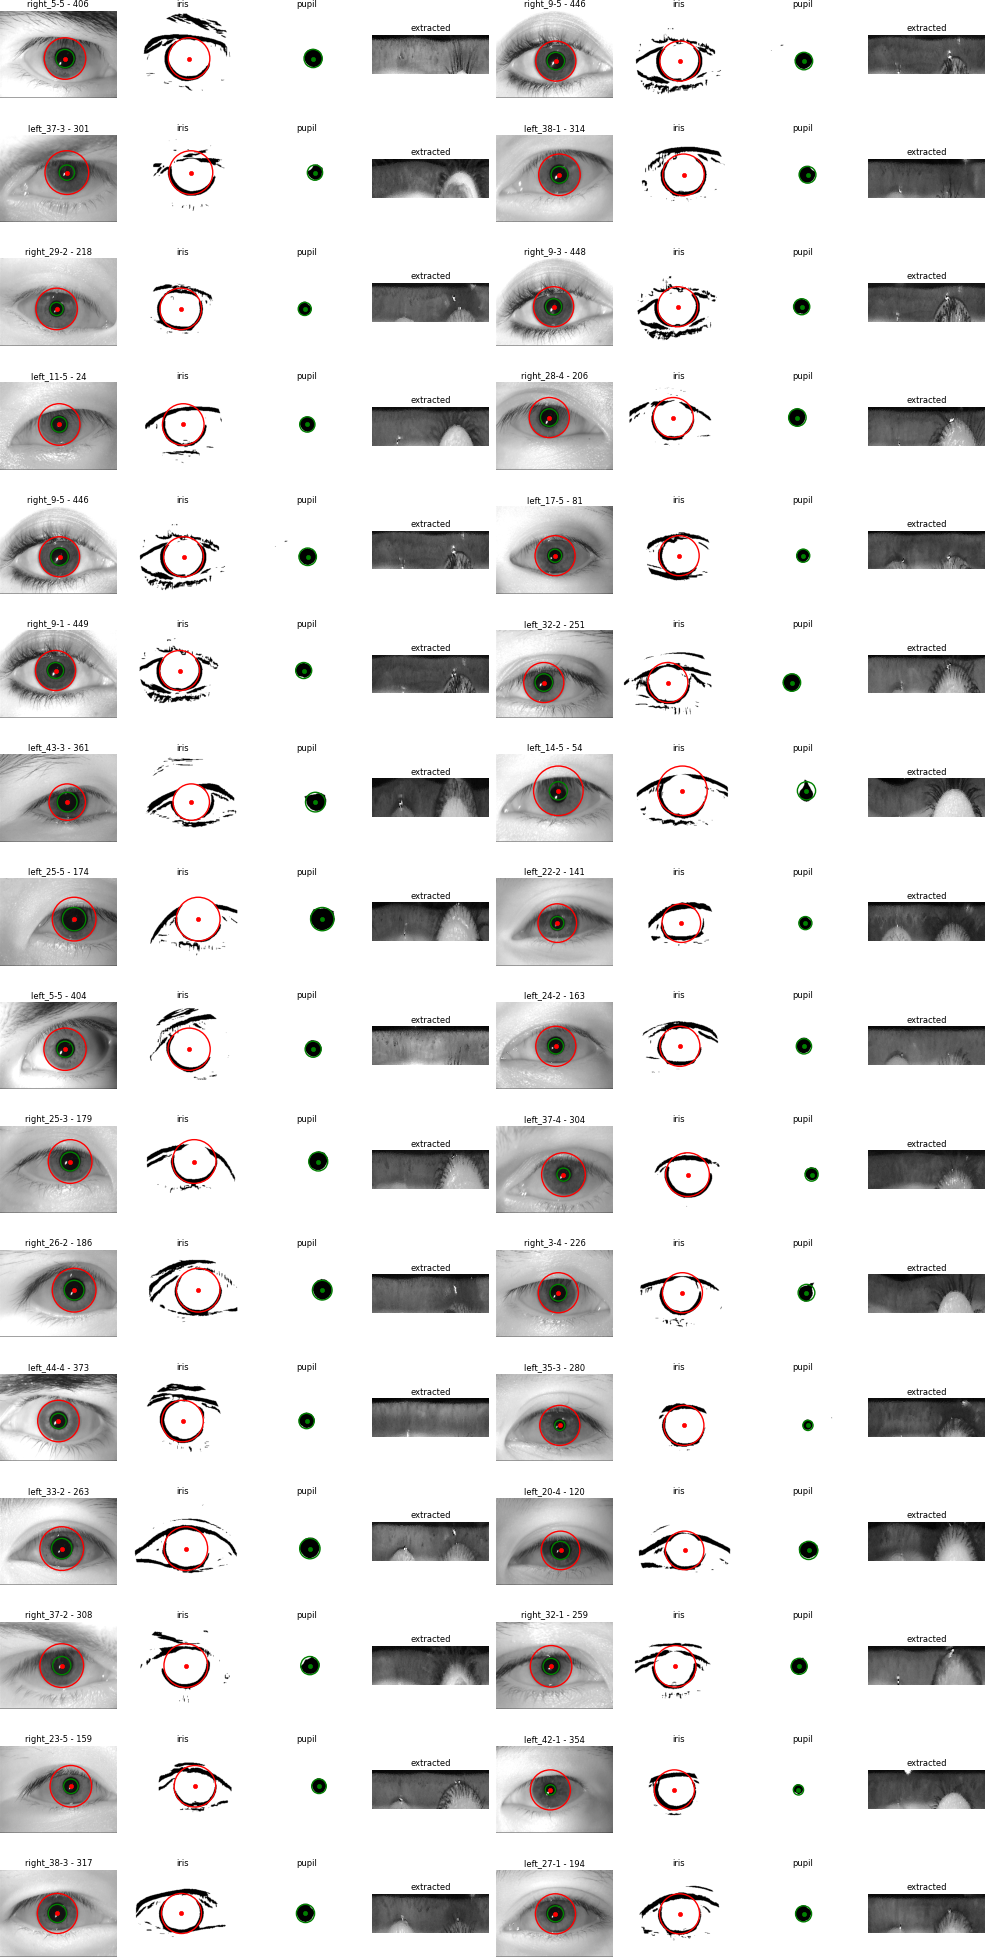
\includegraphics[width=0.7\linewidth]{figures/final_comphrasion.png}
    \caption{Wizualizacja procesu wycinania tęczówki. Widoczne granice źrenicy i tęczówki, ich maski binarne oraz wyodrębniona tęczówka w postaci rozprostowanego obrazu.}
    \label{fig:final_comparison}
\end{figure}

Przekształcone obrazy tęczówek mogą być bezpośrednio wykorzystane do ekstrakcji cech i porównań biometrycznych, takich jak analiza tekstury czy kodowanie wzorców.

\clearpage

\section{Algorytm Daugmana}

\subsection*{Obróbka wstępna}

\begin{figure}[H]
    \centering
    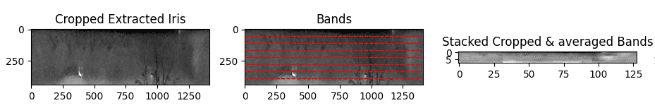
\includegraphics[width=0.9\linewidth]{figures/obrobka wstepna.png}
    \caption{Obróbka wstępna}
\end{figure}

Aby przygotować obraz do dalszej analizy i segmentacji, proces wstępnej obróbki podzielono na trzy zasadnicze etapy:

\begin{enumerate}
  \item \textbf{Przycięcie (crop)}\\
    Na wejściu do algorytmu wykorzystujemy obraz o oryginalnych wymiarach 480 × 1410 pikseli. W celu uniknięcia późniejszej interpolacji przy podziale na równe segmenty, od góry obrazu odcinamy 40 wierszy, uzyskując końcowy rozmiar 470 × 1410 px. Taki zasadniczy wymiar wysokości (440 px) jest wielokrotnością ośmiu, co pozwala na precyzyjny podział bez utraty informacji o obszarze źrenicy.

  \item \textbf{Podział na pasy i wstępne przycięcie kątowe}\\
    Przygotowany obraz dzielimy na 8 poziomych pasów o jednakowej wysokości 55 pikseli (440 ÷ 8 = 55). Następnie, na każdym z pasów, usuwamy fragmenty odpowiadające określonym kątom, zaokrąglając tak, aby szerokość pozostałej części była wielokrotnością 128 pikseli:
    \begin{itemize}
      \item \emph{Pasy 0–3:} usuwamy łącznie ok. 30° obrazu, tak aby pozostała szerokość wynosiła 1280 px.
      \item \emph{Pasy 4–5:} usuwamy po ok. 67° zarówno od góry, jak i od dołu, uzyskując szerokość 768 px.
      \item \emph{Pasy 6–7:} analogicznie usuwamy łącznie ok. 134° (po ok. 67° od góry i od dołu), co daje szerokość 640 px.
    \end{itemize}

  \item \textbf{Uśrednienie radialne}\\
    Z każdej z uzyskanych części obliczamy średnią wartość pikseli w kierunku pionowym, sprowadzając każdy pas do wysokości 1 px oraz szerokości 128 px. W efekcie końcowym otrzymujemy osiem pasów o wymiarach 1 × 128 px, gotowych do dalszej analizy.
\end{enumerate}

\subsection*{Generowanie kodów tęczówki}

\subsection*{Eksperymentalne wyznaczenie częstotliwości}

Istotnym parametrem używanym do identyfikacji osoby, a nie podanym w publikacjach Daugmana, jest częstotliwość. Jej znaczenie demonstrują rysunki \Cref{fig:wpływ_freq_1} oraz \Cref{fig:wpływ_freq_2}. Na pierwszym z nich widać istotny wzrost kodowanej informacji wraz ze wzrostem częstotliwości. Na drugim zaś – jak zmienia się średnia odległość Hamminga wraz ze zmianą częstotliwości. Pomiar ten wykonywany jest poprzez porównanie pierwszego zdjęcia z grupy pięciu zdjęć jednej osoby (kodowane) z pozostałymi oraz z innymi osobami. Dla częstotliwości 0.001 różnice są znikome, natomiast przy wartościach wzrastających do około 0.5 zauważalne stają się istotne rozbieżności. Na tej podstawie przyjęto wartość 0.5 do dalszego przetwarzania.

\begin{figure}[H]
    \centering
    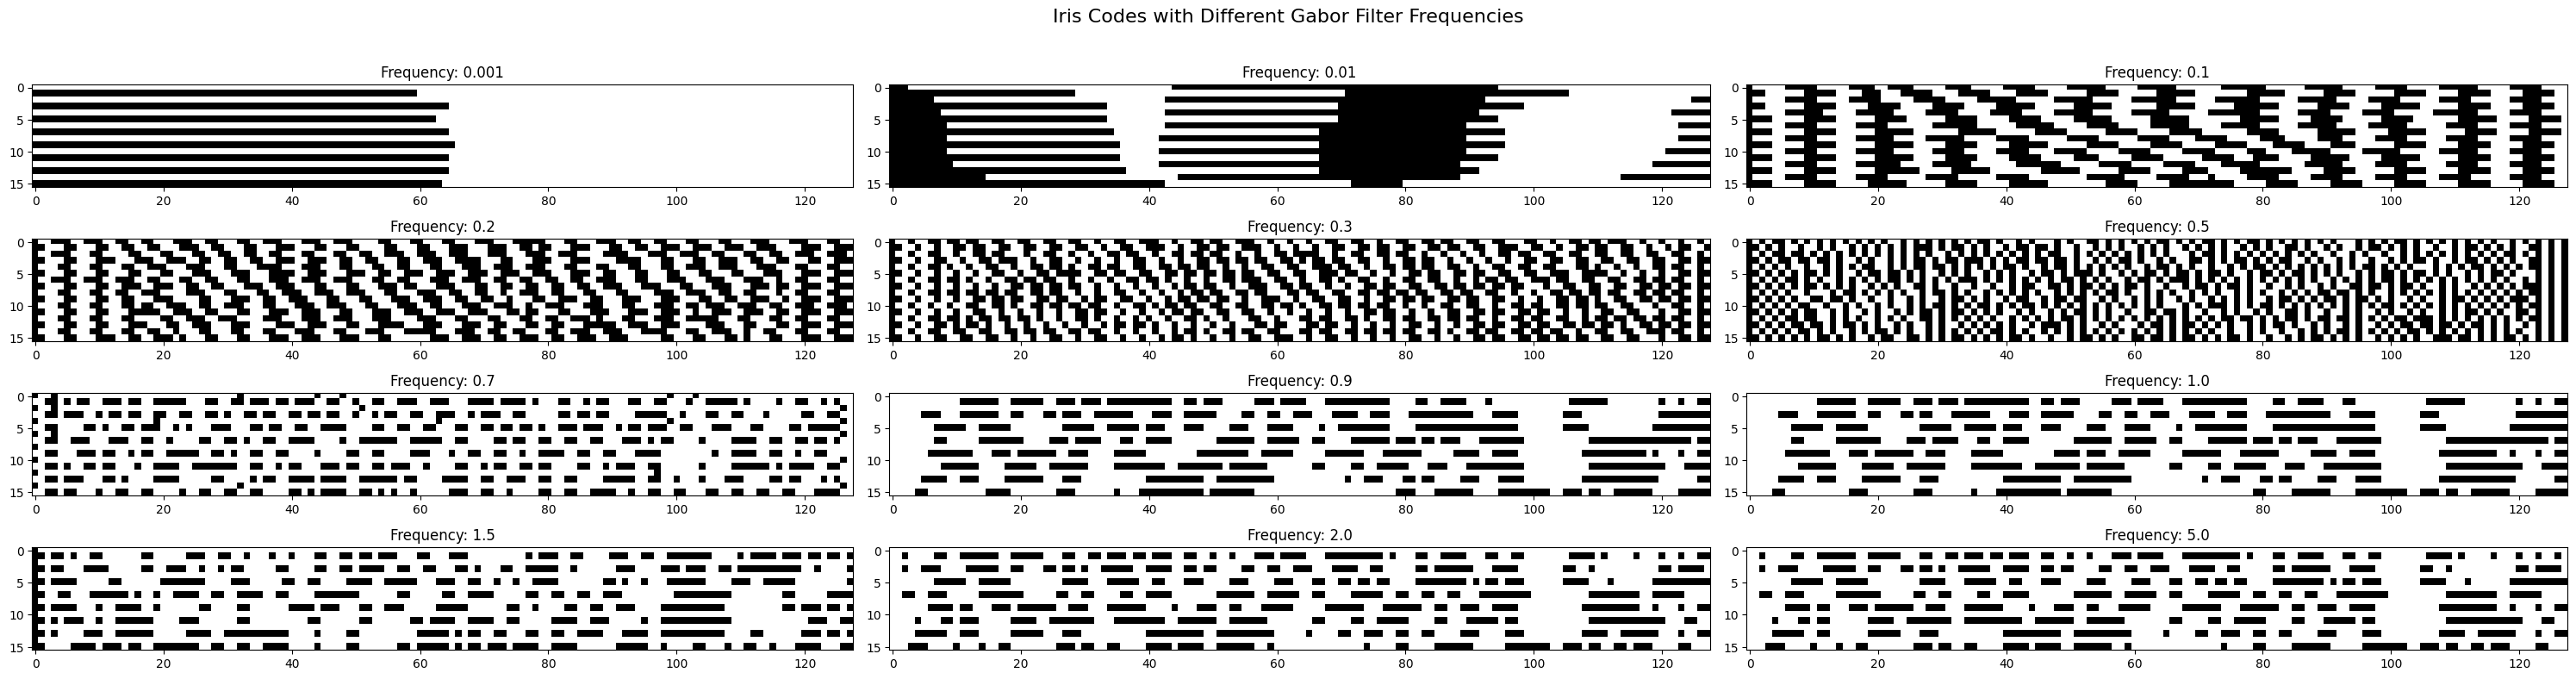
\includegraphics[width=1\linewidth]{figures/waznosc_freq_1.png}
    \caption{Wygląd kodowania na podstawie częstotliwości}
    \label{fig:wpływ_freq_1}
\end{figure}

\begin{figure}[H]
    \centering
    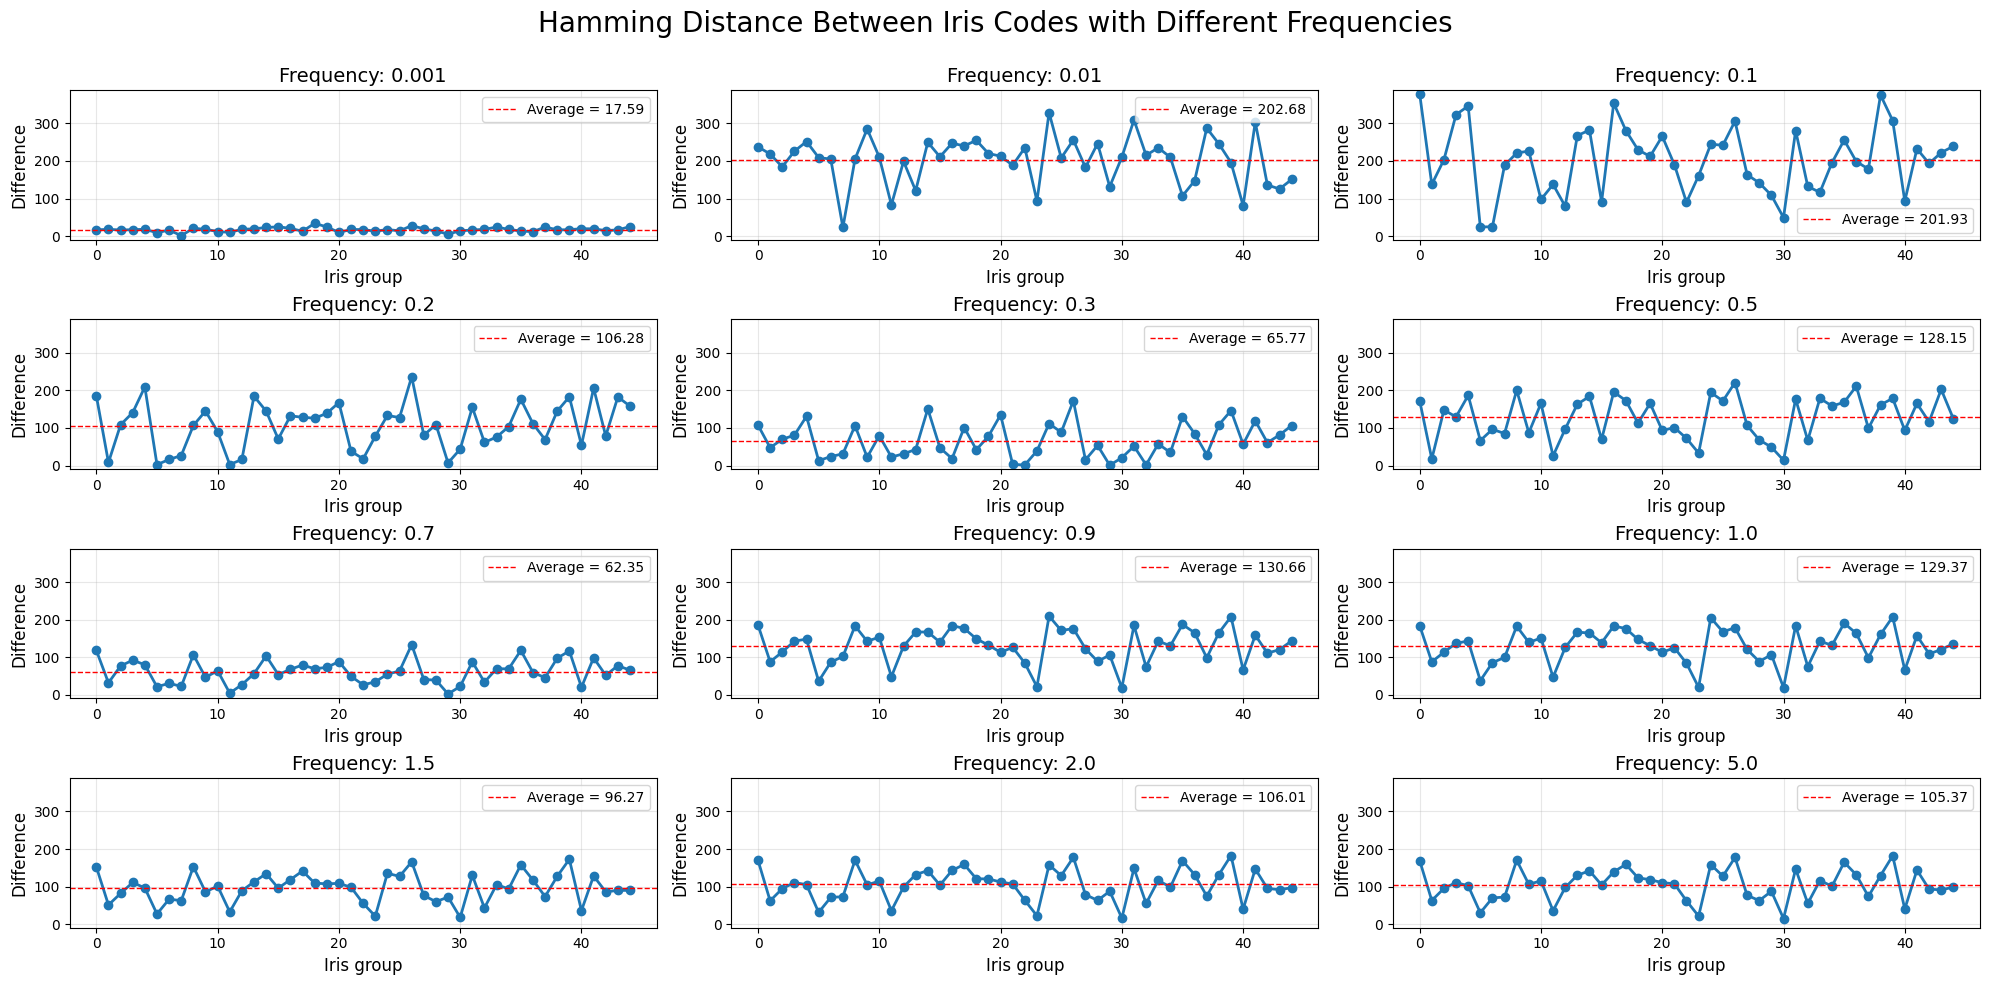
\includegraphics[width=1\linewidth]{figures/waznosc_freq_2.png}
    \caption{Odległość Hamminga między tęczówkami różnych osób}
    \label{fig:wpływ_freq_2}
\end{figure}

\section{Demo}

W tej części przedstawiono wyniki eksperymentów, które potwierdzają, że tęczówka jest skutecznym narządem do identyfikacji biometrycznej.

\subsection*{Ta sama osoba, oko lewe i prawe}

Na poniższym zdjęciu przedstawiono kody tęczówki tej samej osoby, lecz dla dwóch różnych oczu. Zgodnie z hipotezą, wzorce tęczówek lewego i prawego oka powinny się różnić – co wyraźnie widać na obrazie. Białe pola wskazują miejsca rozbieżności pomiędzy kodami, które stanowią około 50

\begin{figure}[H]
    \centering
    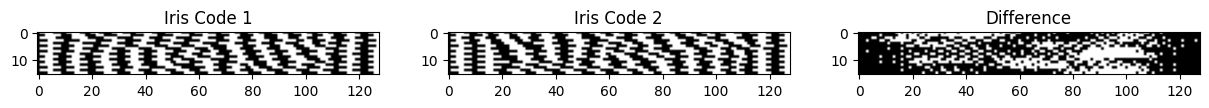
\includegraphics[width=0.75\linewidth]{figures/ta_sama_osoba_lewe_i_prawe.png}
    \caption{Oko lewe i prawe tej samej osoby}
\end{figure}

\subsection*{Ta sama osoba, to samo oko}

Kolejnym przykładem jest porównanie kodów wygenerowanych dla tego samego oka na podstawie dwóch różnych zdjęć. Pomimo różnic warunków rejestracji, wygenerowane kody pozostają do siebie bardzo podobne, co umożliwia skuteczną identyfikację osoby.

\begin{figure}[H]
    \centering
    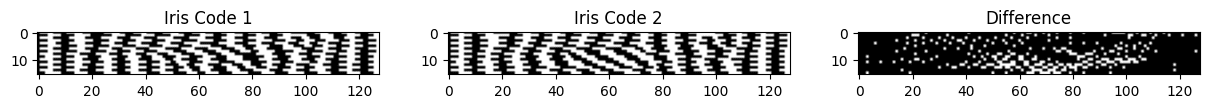
\includegraphics[width=0.75\linewidth]{figures/ta_sama_osoba_to_samo_oko.png}
    \caption{Różne zdjęcia tego samego oka}
\end{figure}

\subsection*{Różne osoby}

Porównanie kodów tęczówek różnych osób wykazuje wyraźne różnice. Na rysunkach \Cref{fig:rozne-osoby} oraz \Cref{fig:to-samo-oko-comparison} widać liczne białe pola, świadczące o braku zgodności pomiędzy kodami, co umożliwia jednoznaczną identyfikację.

\begin{figure}[H]
    \centering
    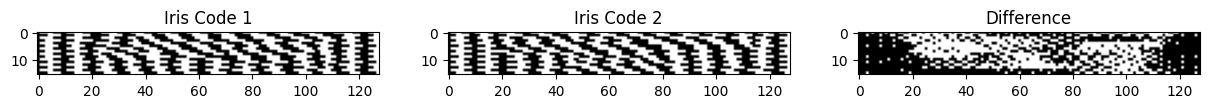
\includegraphics[width=0.75\linewidth]{figures/rozne osoby.png}
    \caption{Kody tęczówki różnych osób}
    \label{fig:rozne-osoby}
\end{figure}

\begin{figure}[H]
    \centering
    \begin{subfigure}[t]{0.48\linewidth}
        \centering
        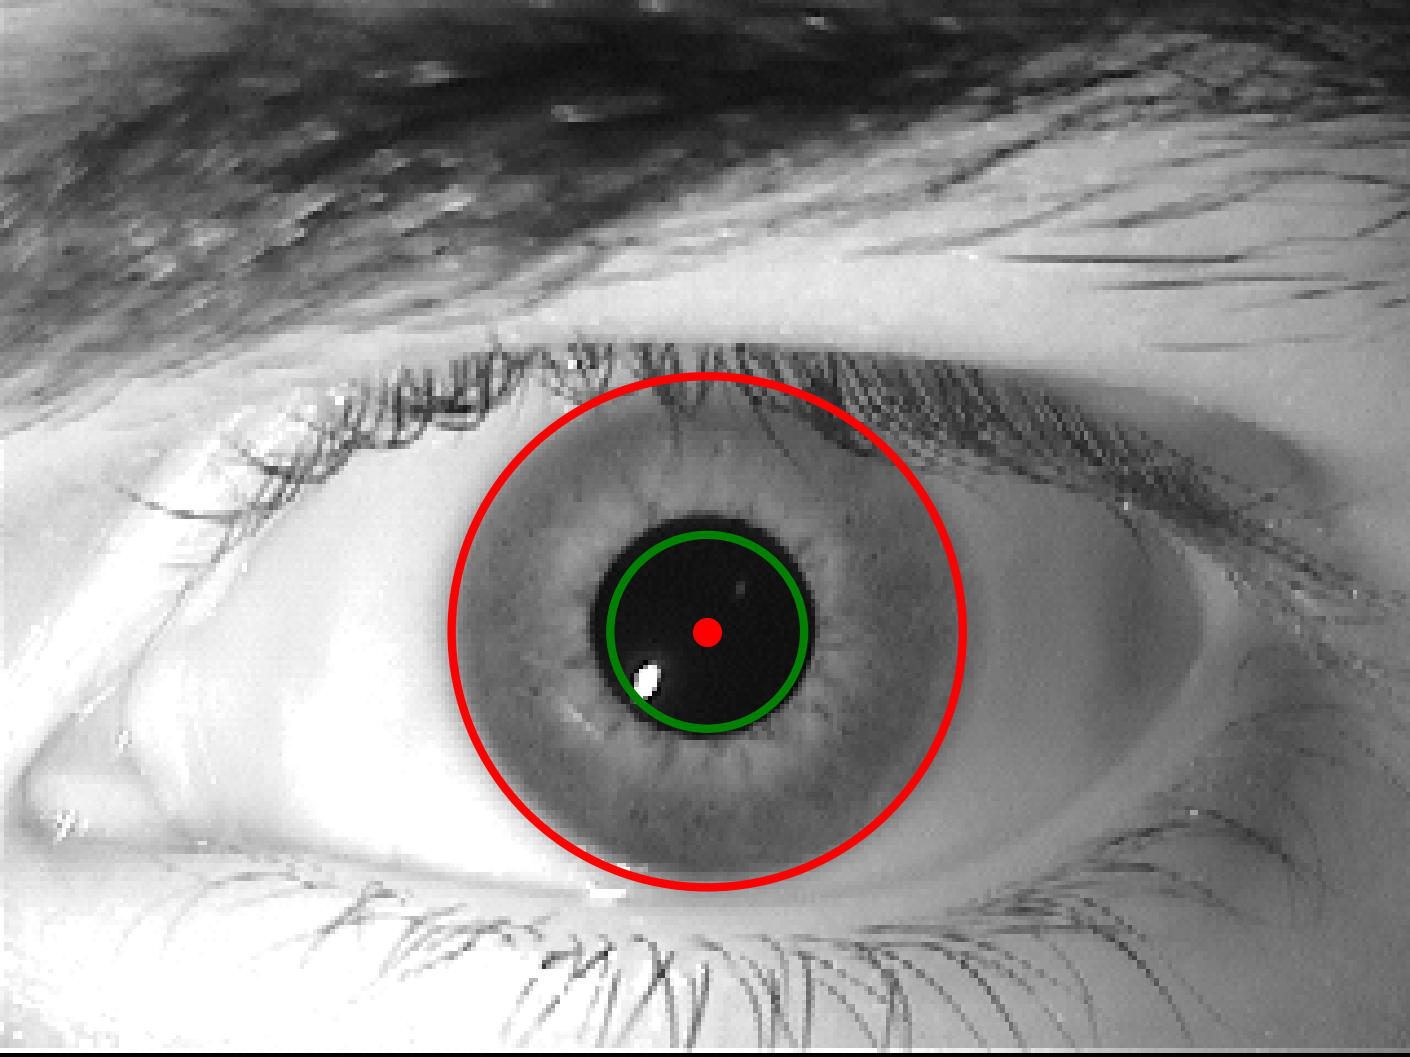
\includegraphics[width=0.75\linewidth]{figures/44-1.png}
        \caption{Zdjęcie 44-1}
    \end{subfigure}
    \begin{subfigure}[t]{0.48\linewidth}
        \centering
        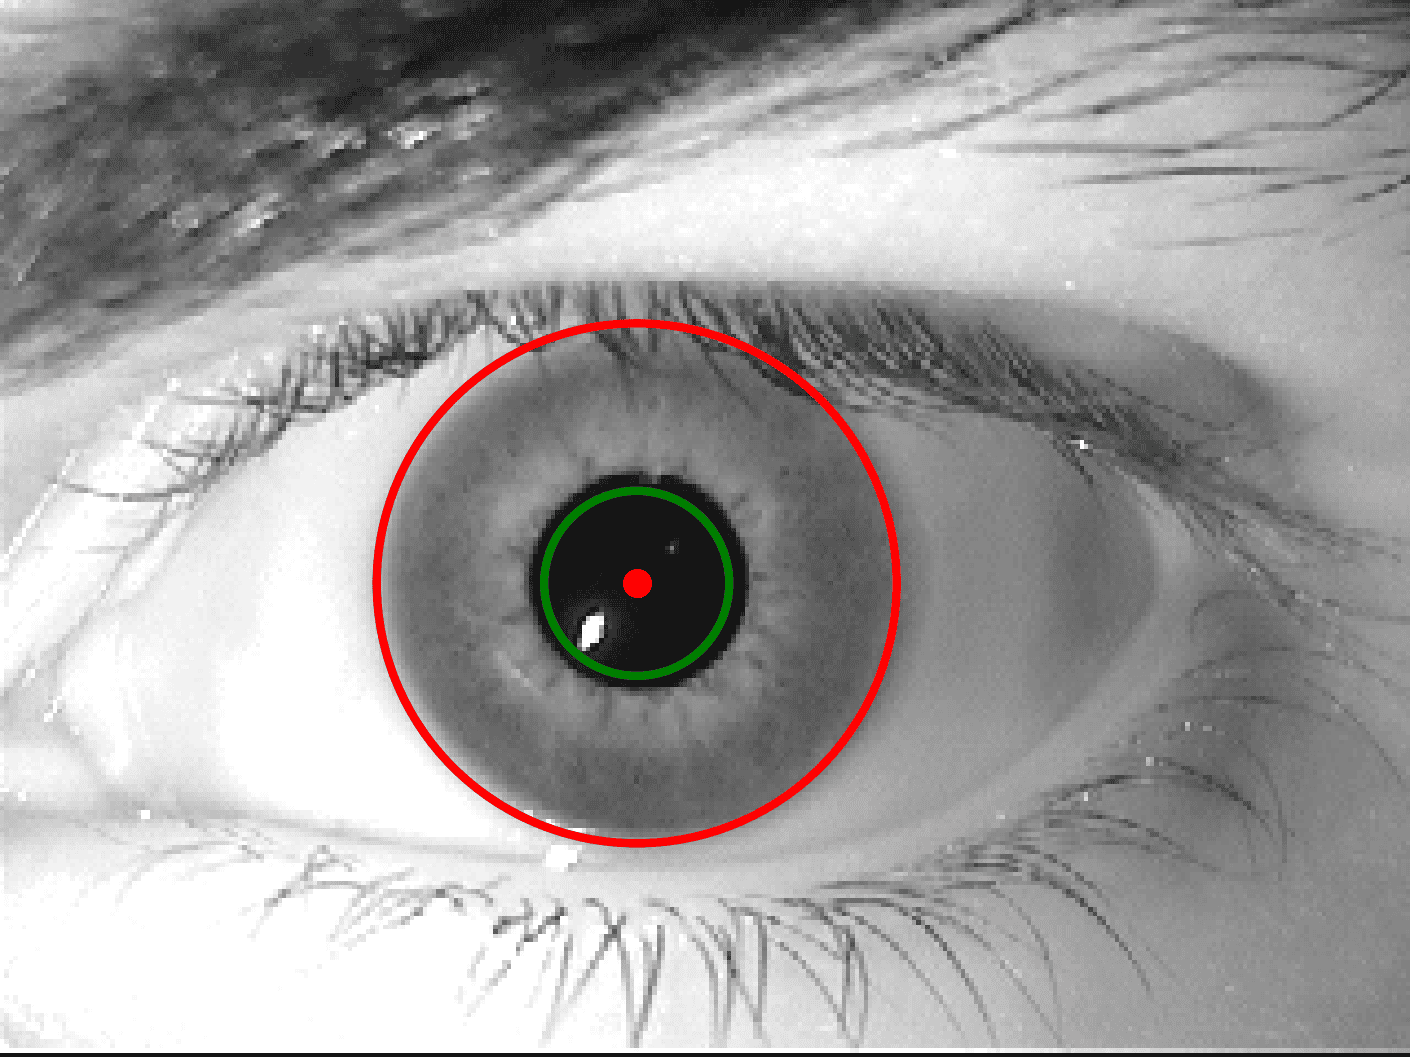
\includegraphics[width=0.75\linewidth]{figures/44-2.png}
        \caption{Zdjęcie 44-2}
    \end{subfigure}
    \caption{To samo oko, ale różne zdjęcia}
    \label{fig:to-samo-oko-comparison}
\end{figure}

\subsection*{Performance tests}

Przeprowadzono prosty test wydajnościowy, z którego wynika, że zakodowanie rozprostowanego obrazu tęczówki zajmuje ok. 0.0039 sekundy, co daje około 253 kodów na sekundę. Samo uzyskanie tego kodu zajmuje średnio 0.0012 sekundy (810 kodów na sekundę). Mimo braku optymalizacji, wydajność systemu jest bardzo wysoka, dając całościową prędkość systemu (licząc wczytywanie zdjęcia do ramu) rzędu 253 kodów na sekundę. Z pewnością dodatkowe optymalizacje mogą poprawić ten wynik jeszcze bardziej.

\section{Podsumowanie}

W projekcie zrealizowano kompletny łańcuch przetwarzania obrazu tęczówki, zgodnie z klasycznym podejściem Johna Daugmana – od surowych zdjęć oka do binarnego \textit{kodu tęczówki} stosowanego w biometrii.

\begin{enumerate}
    \item \textbf{Zbiór danych:}  
          Wykorzystano publiczny zbiór \emph{naureenmohammad/mmu-iris-dataset} (45 osób × 2 oczy × 5 ujęć). Pomimo wyzwań związanych z jakością zdjęć, uzyskano stabilną segmentację.
    \item \textbf{Segmentacja oka:}  
          \begin{itemize}
              \item \emph{Źrenica:} stosowano progowanie po filtrach kontrastu i wyostrzania; projekcje poziome i pionowe ustalają środek i promień.
              \item \emph{Tęczówka:} filtr średni, wzmocnienie kontrastu, filtr Sobela; maskowanie tła i źrenicy; promień wyznaczany z projekcji radialnej, poziomej i pionowej, a następnie uśredniany.
          \end{itemize}
    \item \textbf{Ekstrakcja pierścienia tęczówki:}  
          Wycięto annulus między źrenicą a brzegiem tęczówki i „rozprostowano” go do formy prostokątnej.
    \item \textbf{Algorytm Daugmana:}  
          Po przycięciu obrazu, podziale na osiem pasów i uśrednieniu radialnym, eksperymentalnie ustalono optymalną częstotliwość filtru Gabora na poziomie około 0.5, maksymalizując różnicę Hamminga.
    \item \textbf{Eksperymenty weryfikacyjne:}  
          \begin{itemize}
              \item \textit{Lewe vs prawe oko tej samej osoby:} około 50
              \item \textit{To samo oko, różne zdjęcia:} niskie odległości Hamminga potwierdzają stabilność kodów.
              \item \textit{Różne osoby:} kody znacząco się różnią, umożliwiając jednoznaczną identyfikację.
              \item \textit{Wydajność:} czas generacji kodu wynosi ok. 0.0023 s, co daje ok. 437 kodów/s.
          \end{itemize}
\end{enumerate}

\textbf{Wniosek:} Zaproponowana ścieżka przetwarzania obrazu tęczówki spełnia wymagania systemów biometrycznych, zapewniając wysoką rozróżnialność międzyosobniczą, niską zmienność wewnątrzosobniczą oraz dużą wydajność operacyjną.

\end{document}
